\chapter{Introduction}\label{ch:introduction}
%Structure
% Introduction
% Problem domain & environment
%	- Semester project, cooperation with other groups
% Intention of the solution
%	- Scope
%	- Backend focus, not GUI and aesthetics
%	- Advantages of such a solution
% Transition to problem statement


% Introduction - awesome first sentence
%Commuters are causing traffic jams in dense areas where people are traveling similar routes. \todo{this sentence isn't awesome at all - Claus}
People traveling the same route in different vehicles induce slower traffic and a heavier strain on the environment \cite{trafficJam}\cite{trafficEmissions}.
This project embarks on the task of informing the individual commuters of other commuters traveling a similar path, so that they can share vehicle.
If this project is successful, the reduced number of cars could reduce the CO$_2$ emissions caused by traffic and commuting.

\section{Project environment}
% Problem domain and environment
This project is part of the collaboration project, \gls{astep}, in the SW6F16 semester of Aalborg University.
The project's goal is to develop a location-based service with accompanying applications. 

% Semester project environment + sprint description
The \gls{astep} project was developed in 10 teams with 4 members each in the span of 4 months.
The project was furthermore divided into sprints with each sprint spanning over 4 weeks, making the total number of sprints; 4.
The sprints are synchronization points of the project groups, and this report will contain documentation of each sprint chronologically.

The first sprint is intended for analysis and collaboration development, the second and third are development sprints, and the fourth is intended for testing and finalizing the development.
The 10 project groups are assigned to their respective tasks, with 7 project groups developing the core \gls{astep} service, while the remaining three groups are developing applications utilizing the system.

% group role
\section{Group Role}\label{sec:grouprole}
This section describes the multi-group project setting and defines the role of our group’s work in the multi-group project.

The multi-group project consists of several components, including user management, outdoor location based services, and database groups as seen in Figure \ref{fig:astepGroups}.
OD and ID in the figure are abbreviations of respectively outdoor and indoor location based services.
Each group is assigned to one component and some components have multiple groups assigned to them
The intended component architecture can be seen in Figure \ref{fig:astepCore}.

\begin{figure}[h!]
	\centering
	\begin{subfigure}[b]{0.41\textwidth}
		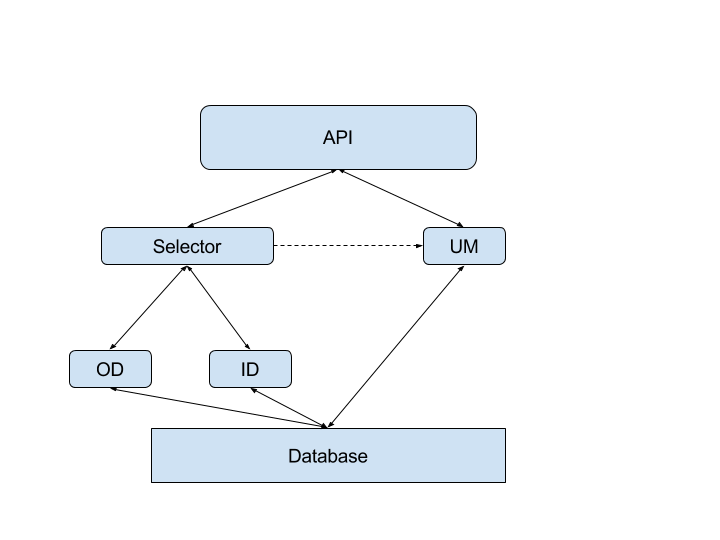
\includegraphics[width=\textwidth,trim={0 0 4cm 0},clip]{figures/InformalArchitecture.png}
		\caption{The \gls{astep} core architecture \cite{astepArchitectureImage}. }
		\label{fig:astepCore}
	\end{subfigure}
	~ %add desired spacing between images, e. g. ~, \quad, \qquad, \hfill etc. 
	%(or a blank line to force the subfigure onto a new line)
	\begin{subfigure}[b]{0.56\textwidth}
		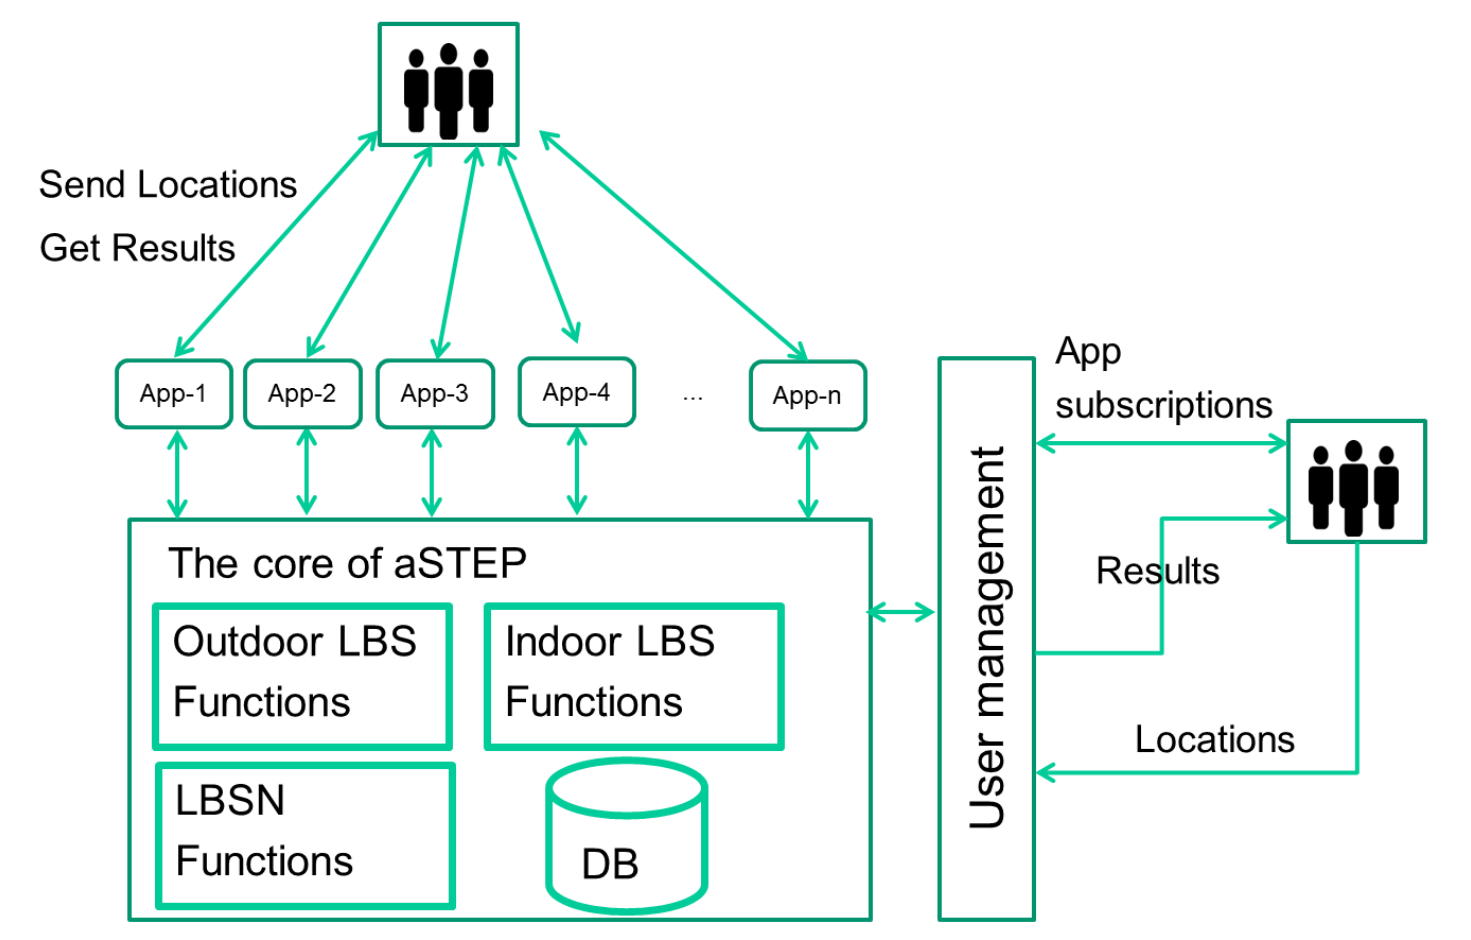
\includegraphics[width=\textwidth]{figures/astepGroups.png}
		\caption{The \gls{astep} group distribution according to the project guidelines.}
		\label{fig:astepGroups}
	\end{subfigure}
	\caption{\gls{astep} architectural design}
	\label{fig:astepArchitecture}
\end{figure}

Our project group is responsible for developing an app that utilizes the \gls{astep} core through the API, and contribute to the development of the interface of the core.
As the project focus is on commuting, the solution will depend upon outdoor location based services.
Any user registration, login or other user related tasks should be handled by the user management group.
According to our project focus and the component architecture, represented in Figure \ref{fig:astepCore}, we will mainly cooperate with the OD and user management groups.



\section{Problem domain}
% Solution scope and definition
\gls{astep}'s planned functionality gave the idea of a large set of location data which a system could use to identify and help drivers and passengers with arranging ridesharing.
The solution's goal is to provide ridesharing suggestions to the users of the solution.
When referring to the term ridesharing in this report, it is referred to as the action of private persons sharing a car for the whole or a part of a route. 
This definition is covered by the terms carpool and ad-hoc ridesharing by \citet{doi:10.1080/01441647.2011.621557}.  

% Intention of the solution
The intention of this project is to develop an Android app that utilizes the \gls{astep} system for historical location data and arranging carpool style ridesharing.
The extent of such a project can be wide and therefore we early choose that the main focus will be to design and implement a basic system, which could be expanded upon in a potential future project.
The purpose of the solution is to propose appropriate candidates for ridesharing to the users of the app.
The project will include developing and implementing of an algorithm that assesses if two users of the system should be suggested for ridesharing.
Other parts of the application, such as graphical user interface, are not prioritized but are developed to be sufficiently functional for practical purposes and testing.

% Solution contributions/advantages
The suggested app could be beneficial in several ways.
There could be environmental and economical savings, as the number of driven polluting cars  is reduced, as described in \cite{doi:10.1080/01441647.2011.621557}.
The app could also decrease problems such as traffic jam and thereby also be time-saving, and causing less frustration for the drivers.

The potential benefits are both social, environmental and economical, as the app allows people meet each other and thus reduce the use of cars, gasoline and the load on the road system.
The future aspect of this solution seems bright since it easily should be modifiable for future transportation needs, i.e. autonomous vehicles.

% Transition to problem statement
To formally define the problem, to initiate research and development, a concrete problem formulation is made.